\subsection{Infraestructura y herramientas}
\subsubsection{Descripción general de la infraestructura}
La infraestructura y las herramientas son la base sobre la que se construirán
los diferentes proyectos de aprendizaje automático. Se encargan de proporcionar
un entorno de desarrollo e investigación eficiente, que permita a los miembros
del equipo centrarse en el desarrollo de modelos sin tener que preocuparse por
la configuración. Concretamente, se han desplegado dos plataformas 
que vienen a cubrir varias de las necesidades fundamentales de los proyectos
como son la gestión y exploración de datasets, la monitorización de experimentos o
el almacenamiento de modelos de inteligencia artificial. Además, se ha añadido un sistema de autenticación 
para garantizar la seguridad y privacidad de los datos.\medskip

Esta infraestructura se ha desplegado en un servidor interno de la empresa
utilizando contenedores de Docker. La elección de esta tecnología se debe a
que permite la creación de entornos aislados y portables, lo que facilita el
despliegue de las aplicaciones. Se ha utilizado Docker Compose para
sincronizar el despliegue de los diferentes servicios, lo que permite
realizar despliegues automatizados mediante las acciones de GitLab CI. La
figura \ref{fig:internal-server} muestra una vista general de la infraestructura
desplegada en el servidor interno de la empresa, donde se pueden observar
como se integran los diferentes servicios y sus respectivas conexiones. Además,
se puede observar que todos los servicios están interconectados mediante un
proxy inverso mediante Nginx, que se encarga de redirigir las peticiones en 
función de la URL. Esto permite que todos los servicios sean
accesibles desde el exterior a través de un único punto de entrada y que el
sistema de autenticación sea común para todos ellos.

\begin{figure}[ht]
    \centering
    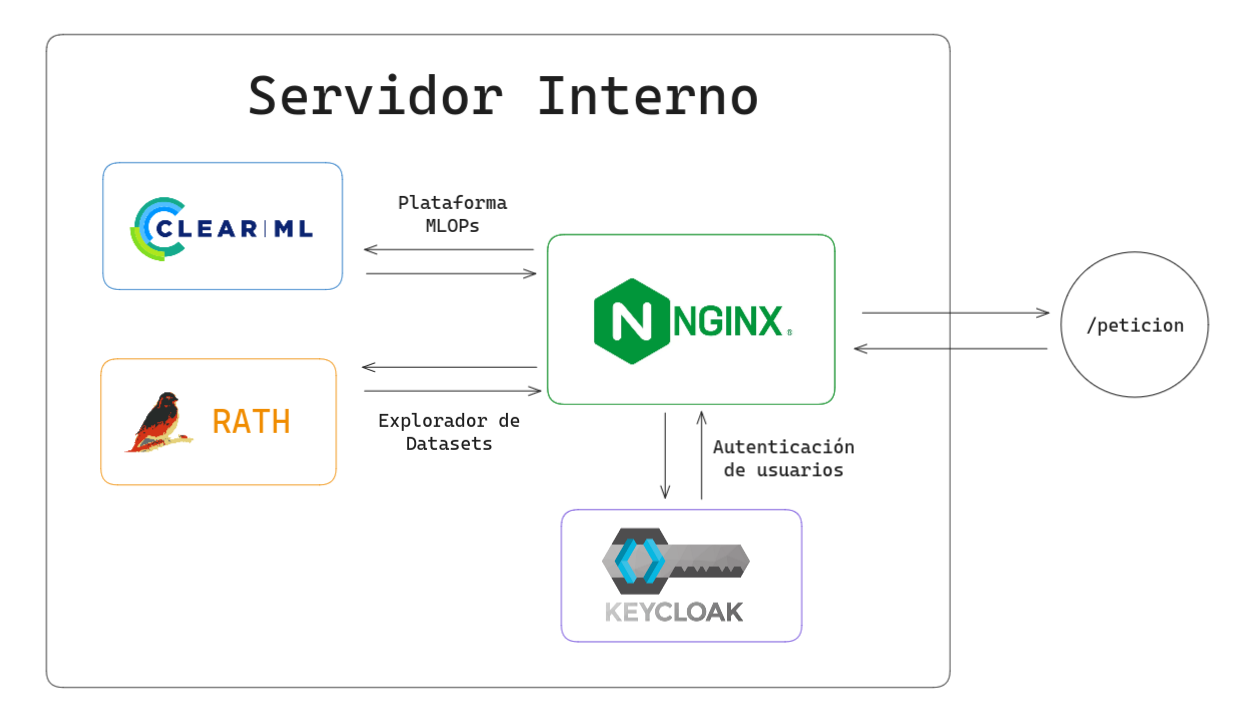
\includegraphics[width=\textwidth]{internal-server.png}
    \caption{Vista general del proyecto}\label{fig:internal-server}
\end{figure}

\subsubsection{Selección de plataformas}
Previo a la elección de las plataformas integradas, se realizó una evaluación
a nivel de equipo para determinar las necesidades que se debían cubrir. Se
identificaron las siguientes funcionalidades fundamentales:

\begin{itemize}
    \item \textbf{F1:} Versionado y almacenamiento de dataset.
    \item \textbf{F2:} Monitorización de experimentos.
    \item \textbf{F3:} Almacenamiento de modelos de inteligencia artificial.
    \item \textbf{F4:} Integración de métricas en datasets y visualización de resultados.
    \item \textbf{F5:} Exploración de datasets.
\end{itemize}

Una vez identificadas las necesidades, se consensuó un criterio de selección
para las plataformas integradas. Este criterio es un criterio de mínimos, es
decir, se seleccionarán las plataformas que cumplan con el criterio mínimo
establecido y que, además, ofrezcan funcionalidades adicionales que puedan
ser de utilidad para el equipo. El criterio de selección se basa en los
siguientes aspectos: 

\begin{itemize}
    \item \textbf{C1 (Facilidad de uso):} Se valora muy positivamente la facilidad de uso de las
    plataformas, ya que se considera que no todo el equipo no tiene experiencia
    previa en el uso de estas herramientas.
    \item \textbf{C2 (Integración con otras herramientas):} Es fundamental que las
    plataformas integradas sean compatibles con las librerías y herramientas
    que se utilizan generalmente en proyectos (TensorFlow, PyTorch, etc.).
    \item \textbf{C3 (Poca dependencia sobre la infraestructura):} Medimos la dependencia
    sobre una plataforma como el numero de acciones que se deben realizar para
    migrar un proyecto vanilla, es decir, un proyecto que no ha sido
    desarrollado con la plataforma en mente. Y penalizando aquellas practicas
    que sean propias de la plataforma y que no sean comunes en la industria.
\end{itemize}

Con estos criterios en mente, se tuvieron en cuenta las siguientes
plataformas a la hora de realizar la evaluación: MLflow, ClearML, Kedro, ZenML, Data Version Controller (DVC),
Rath, Apache Superset. Cada una de estas plataformas tiene diferentes enfoques y 
funcionalidades, pero todas ellas cubren una o varias de las necesidades fundamentales
identificadas, por lo que se consideraron candidatas para su integración en la
infraestructura. La infraestructura final se compondrá de una o varias de estas
plataformas en función de los criterios previamente establecidos. En el estado del arte, se 
muestra un análisis detallado de las plataformas evaluadas y las funcionalidades que ofrecen.\medskip


\begin{table}[ht]
    \centering 
    \begin{tabular}{lccccccccc}  
        
        \toprule
        \multirow{2}{*}{\parbox[c]{.2\linewidth}{\centering Tecnología}} & 
        \multicolumn{5}{c}{\textbf{Funcionalidades}} && 
        \multicolumn{3}{c}{\textbf{Criterios}} \\ 
        
        \cmidrule{2-6} \cmidrule{8-10}
        & {\centering F1} & {F2} & {F3}& {F4} & {F5} && {C1} & {C2} & {C3}\\
        
        \midrule
        MLflow           & --     & \check & \check & --     & --     && \check & \check & \check \\
        ClearML          & \check & \check & \check & \check & --     && \check & \check & \check \\
        DVC              & \check & \check & \check & \check & --     && --     & \check & --     \\ 
        ZenML            & --     & \check & \check & --     & --     && \check & \check & \check \\  
        Kedro            & --     & --     & --     & --     & --     && --     & --     & --     \\ 
        Rath             & --     & --     & --     & --     & \check && \check & --     & \check \\ 
        Apache Superset  & \check & --     & --     & \check & --     && --     & --     & \check \\ 
        Grafana          & \check & --     & --     & \check & --     && --     & --     & \check \\ 
        \bottomrule
        
    \end{tabular}
    \caption{Tabla comparativa de las plataformas evaluadas}
    \label{tab:comparative-table} 
\end{table}

Para finalizar con la evaluación, se puede observar en la tabla \ref*{tab:comparative-table} 
una comparativa que muestra
las funcionalidades y criterios que cumple cada una de ellas de forma resumida.
De acuerdo con la evaluación realizada, se ha decidido integrar ClearML y Rath
en la infraestructura como las plataformas finales. ClearML cubre la mayoría de
las necesidades fundamentales identificadas, ya que ofrece soluciones para la
mayoría de casos de uso, mientras que Rath complementa con la exploración de
datasets de forma sencilla e intuitiva.  

\subsubsection{Seguridad y priviacidad}
La seguridad y la privacidad de los datos son aspectos fundamentales dentro
de un entorno de trabajo empresarial, donde la confidencialidad de los datos
es una prioridad para la empresa. Por ello, ya que ClearML y Rath no cuentan
con un sistema de autenticación robusto, se ha decidido implementar un sistema
de autenticación utilizando Keycloak, que es una solución de código abierto
para la gestión de acceso. Keycloak permite a los usuarios autenticarse con
cuentas de usuario gestionadas por la empresa, lo que garantiza que solo los
usuarios autorizados puedan acceder a los datos. Además, ofrece integraciones
con diferentes proveedores de identidad, lo que facilita la gestión de
usuarios y la integración con otras herramientas.\medskip

Debido a que tanto ClearML como Rath no tienen integraciones directas con
Keycloak, se ha decidido utilizar Nginx como proxy inverso para redirigir
las peticiones a los servicios de ClearML y Rath. De esta forma, se puede
utilizar Keycloak para autenticar a los usuarios y garantizar la seguridad
y la privacidad de los datos. La figura \ref{fig:internal-server} muestra
cómo se ha integrado Keycloak en la infraestructura, así como las conexiones
entre los diferentes servicios y el proxy inverso. En el momento actual, se
ha implementado un sistema de autenticación básico, pero se espera que en el
futuro este sistema se sincronice con el sistema de autenticación de Tecnalia
para una mayor comodidad por parte de los usuarios.

\subsubsection{Despligue Automatizado}
Para la automatización del despliegue de la infraestructura se ha utilizado
GitLab CI, que es una herramienta de integración y despliegue continuo que
permite automatizar el proceso de despliegue de aplicaciones. GitLab CI
permite definir un conjunto de pasos que se ejecutarán cada vez que se
realice un cambio en el repositorio, lo que facilita el despliegue de
aplicaciones y la gestión de la infraestructura.\medskip

Para poder utilizar GitLab CI, es necesario primero definir un runner, que
es un agente que se encarga de ejecutar los pasos definidos en el archivo
de configuración. En este caso, el runner se ha desplegado en el servidor
lo que permite ejecutar los diferentes flujos en el mismo entorno. Además,
otro aspecto a tener en cuenta es que por seguridad, se ha configurado el
sistema con variables de entorno que enmascaran las credenciales de acceso
a los diferentes servicios, lo que garantiza que las credenciales no se
almacenen en el repositorio. En cuanto a las pipelines, se han definido 
tres diferentes flujos para automatizar cada uno de los procesos de 
instalación y actualización:

\begin{itemize}
    \item \textbf{Instalación de autenticación:} Se encarga de instalar Keycloak
    en el servidor junto con la base de datos. Este flujo se ejecutará si no
    se ha instalado Keycloak previamente.
    \item \textbf{Instalación de infraestructura:} Se encarga de instalar ClearML y Rath
    en el servidor. Además, también se encarga de configurar el proxy inverso
    para redirigir las peticiones a los servicios de ClearML y Rath. Este flujo
    se ejecutará si no se ha instalado ClearML previamente.
    \item \textbf{Despliegue de infraestructura:} Se encarga de actualizar el
    servidor a los nuevos cambios realizados en el repositorio. Este flujo se
    lanza cada vez que detecta un cambio en el repositorio, pero requiere de
    una aprobación manual para ejecutarse.
\end{itemize}

La idea de estos flujos es que se puedan ejecutar de forma independiente
y que en caso de que se necesite realizar un cambio en la infraestructura,
se pueda lanzar el flujo en otro servidor para instalar la infraestructura
de forma automática. Además, facilita el trabajo en local, ya que una vez
automatizado el despliegue, los cambios en local se pueden probar lanzar
directamente en el servidor.

\subsubsection{Problemas durante el Despliegue}
A continuación se detallan la lista de problemas que se han encontrado durante
el despliegue de la infraestructura y las soluciones que se han aplicado para
resolverlos. Estos soluciones se detallan con el fin de que puedan ser de utilidad
para futuros despliegues o como registro para mejoras futuras.

\begin{itemize}
    \item \textbf{Clearml no es compatible con servidores no IPv6.} Por defecto,
    ClearML utiliza direcciones IPv4 e IPv6 para comunicarse con el servidor. Sin
    embargo, en el servidor interno de la empresa no está habilitado el soporte
    para direcciones IPv6, lo que provoca que ClearML no pueda comunicarse con el
    servidor. Internamente, ClearML utiliza una configuración de Nginx para esta
    comunicación, pero no es posible modificarla directamente ya que el contenedor de
    Docker lanza un script en bash que sobrescribe la configuración de Nginx y luego lanza
    el servidor. La solución a este problema es sobrescribe una variable interna llamada
    \textit{DISABLE\_NGINX\_IPV6} dentro del contenedor de Webserver de ClearML. Este
    error es común pero no está documentado en la documentación oficial, la solución
    es una propuesta personal que ha sido descubierta mediante la lectura del código.
    \item \textbf{ClearML no renderiza correctamente en el navegador.} Otro de los problemas
    que encontramos al desplegar ClearMl es que el servidor interno de la empresa no
    era capaz de servir archivos estáticos de un tamaño superior a 3.5MB. Esto provocaba
    que la interfaz de usuario de ClearML no se renderizara correctamente los gráficos,
    ya que internamente utiliza plotly para la visualización de los mismos. La solución
    a este problema fue recompilar la libreria de plotly por nuestra cuenta incluyendo
    solamente los gráficos que necesitamos, de esta forma reducimos el tamaño de los
    archivos estáticos y conseguimos que la interfaz de usuario se renderizara correctamente.
\end{itemize}